\section{Über-/Untersteuerung und Seitenkraftbeiwerte}
\subsection{Über-/Untersteuerung}
Ob das Auto über- oder untersteuert, kann bei einer Kreisfahrt  untersucht werden. Wir haben festgestellt, dass sich der Radius des Kreises, auf dem sich das Auto bewegt, beim Erhöhen der Geschwindigkeit vergrößert. Dies spricht für ein \textbf{Untersteuern} des Fahrzeuges.

\subsection{Seitenkraftbeiwerte}

Um die Seitenkraftbeiwerte abzuschätzen, haben wir eine Keisfahrt mit konstanter Geschwindigkeit $v=1.66\frac{m}{s}$ auf einem Kreis mit Radius $R=0.84m$ durchgeführt. Der gemittelte Vorderradwinkel betrug $\delta_V=22.5^\circ$. Bei einer solchen Kreisfahrt ist die zweite Ableitung der Gierrate $\ddot{\Psi}$ und die erste Ableitung des Schwimmwinkels $ \beta$ null. Außerdem ist $\dot{\Psi}=\frac{v}{R}$ und $\beta$ konstant. Wenn man nun noch zusätzlich annimmt, dass $S_L=M_{LZ}=0$ gilt, vereinfacht sich die lineare Bewegungsgleichung
$$ \begin{bmatrix} 
mv^2 & 0 \\
0 & I 
\end{bmatrix} 
\begin{bmatrix} 
\dot{\beta} \\
\ddot{\Psi}
\end{bmatrix}+ 
\begin{bmatrix} 
mv+k_{SV}l_V-k_{SH}l_{H} \\
\frac{k_{SV}l_V^2+k_{SH}l_H^2}{v}  
\end{bmatrix} \dot{\Psi}+
\begin{bmatrix} 
k_{SV}+k_{SH} \\
k_{SV}l_V-k_{SH}l_H 
\end{bmatrix} \beta=
\begin{bmatrix} 
S_L+k_{SV}\delta_v \\
M_{LZ}+k_{SV}l_V\delta_V 
\end{bmatrix}
$$
auf 
$$  
\begin{bmatrix} 
mv+k_{SV}l_V-k_{SH}l_{H} \\
\frac{k_{SV}l_V^2+k_{SH}l_H^2}{v}  
\end{bmatrix} \frac{v}{R}+
\begin{bmatrix} 
k_{SV}+k_{SH} \\
k_{SV}l_V-k_{SH}l_H 
\end{bmatrix} \beta=
\begin{bmatrix} 
k_{SV}\delta_V \\
k_{SV}l_V\delta_V 
\end{bmatrix}.
$$
Wenn man diese nach $k_{SH}$ beziehungsweise $k_{SV}$ umstellt, erhält man 
$$
K_{SH}=\frac{l_V mv^2}{l(l_H-R\beta)} \qquad \qquad K_{SV}=\frac{l_H}{l^2\frac{R\delta_V-l}{mlv^2}+\frac{l_V}{K_{SH}}}.
$$
Aus vorherigen Versuchen sind folgende Parameter bekannt:

$m=2.2061 kg,l_V=0.1421 m,l_H=0.1195 m,l=0.261 m$. Um $K_{SH}$ zu bestimmen wird nun also nur noch der Schwimmwinkel benötigt. Da dieser sehr klein ist und das Auto auf den Aufnahmen der Kreisfahrt nicht sonderlich scharf ist, ist es nicht einfach diesen exakt zu messen. Um eine grobe Idee zu bekommen, wo er liegen könnte, kann man die rote Tangente des Kreises betrachten (\ref{fig:Kreis}), auf dem sich das Auto bewegt. Auf dieser Tangente liegt der Geschwindigkeitsvektor $v$ des Autos. Die blaue Linie zeigt in die Richtung, in die das Auto zeigt. Der Schwimmwinkel ist nun der Winkel zwischen diesen beiden Linien. 

Da bei der Bestimmung der Seitenkraftbeiwerte der Fehler von $\beta$ den größten Einfluss hat, werden die vergleichsweise geringen Fehler der anderen Parameter vernachlässigt. Je nachdem wo $\beta$ tatsächlich liegt, ergeben sich folgende Parameter:

\begin{center}
\begin{figure}[h]
\begin{subfigure}{.5\textwidth}
	\centering
	\begin{tabular}{|c|c|c|c|}
\hline
$\beta$ in Grad & $k_{SH}$& $k_{SV}$&$k_{SH}l_H-k_{SV}l_V$ \\\hline

%-1  & 22.61 & 12.96&0.86\\\hline
0  & 28.18 & 14.97&1.24\\\hline
1  & 32.14 & 16.24&1.53\\\hline
2  & 37.39 & 17.73&1.95\\\hline
3  & 44.70 & 19.53&2.57\\\hline
4  & 55.56 & 21.74&3.55\\\hline
4.4  & 61.54 & 22.77&4.12\\\hline
5  & 73.38 & 24.51&5.29\\\hline

\end{tabular}
	\caption{Seitenkraftbeiwerte}
	\label{fig:Seitenkraftbeiwerte}
\end{subfigure}
\begin{subfigure}{.4\textwidth}
	\centering
	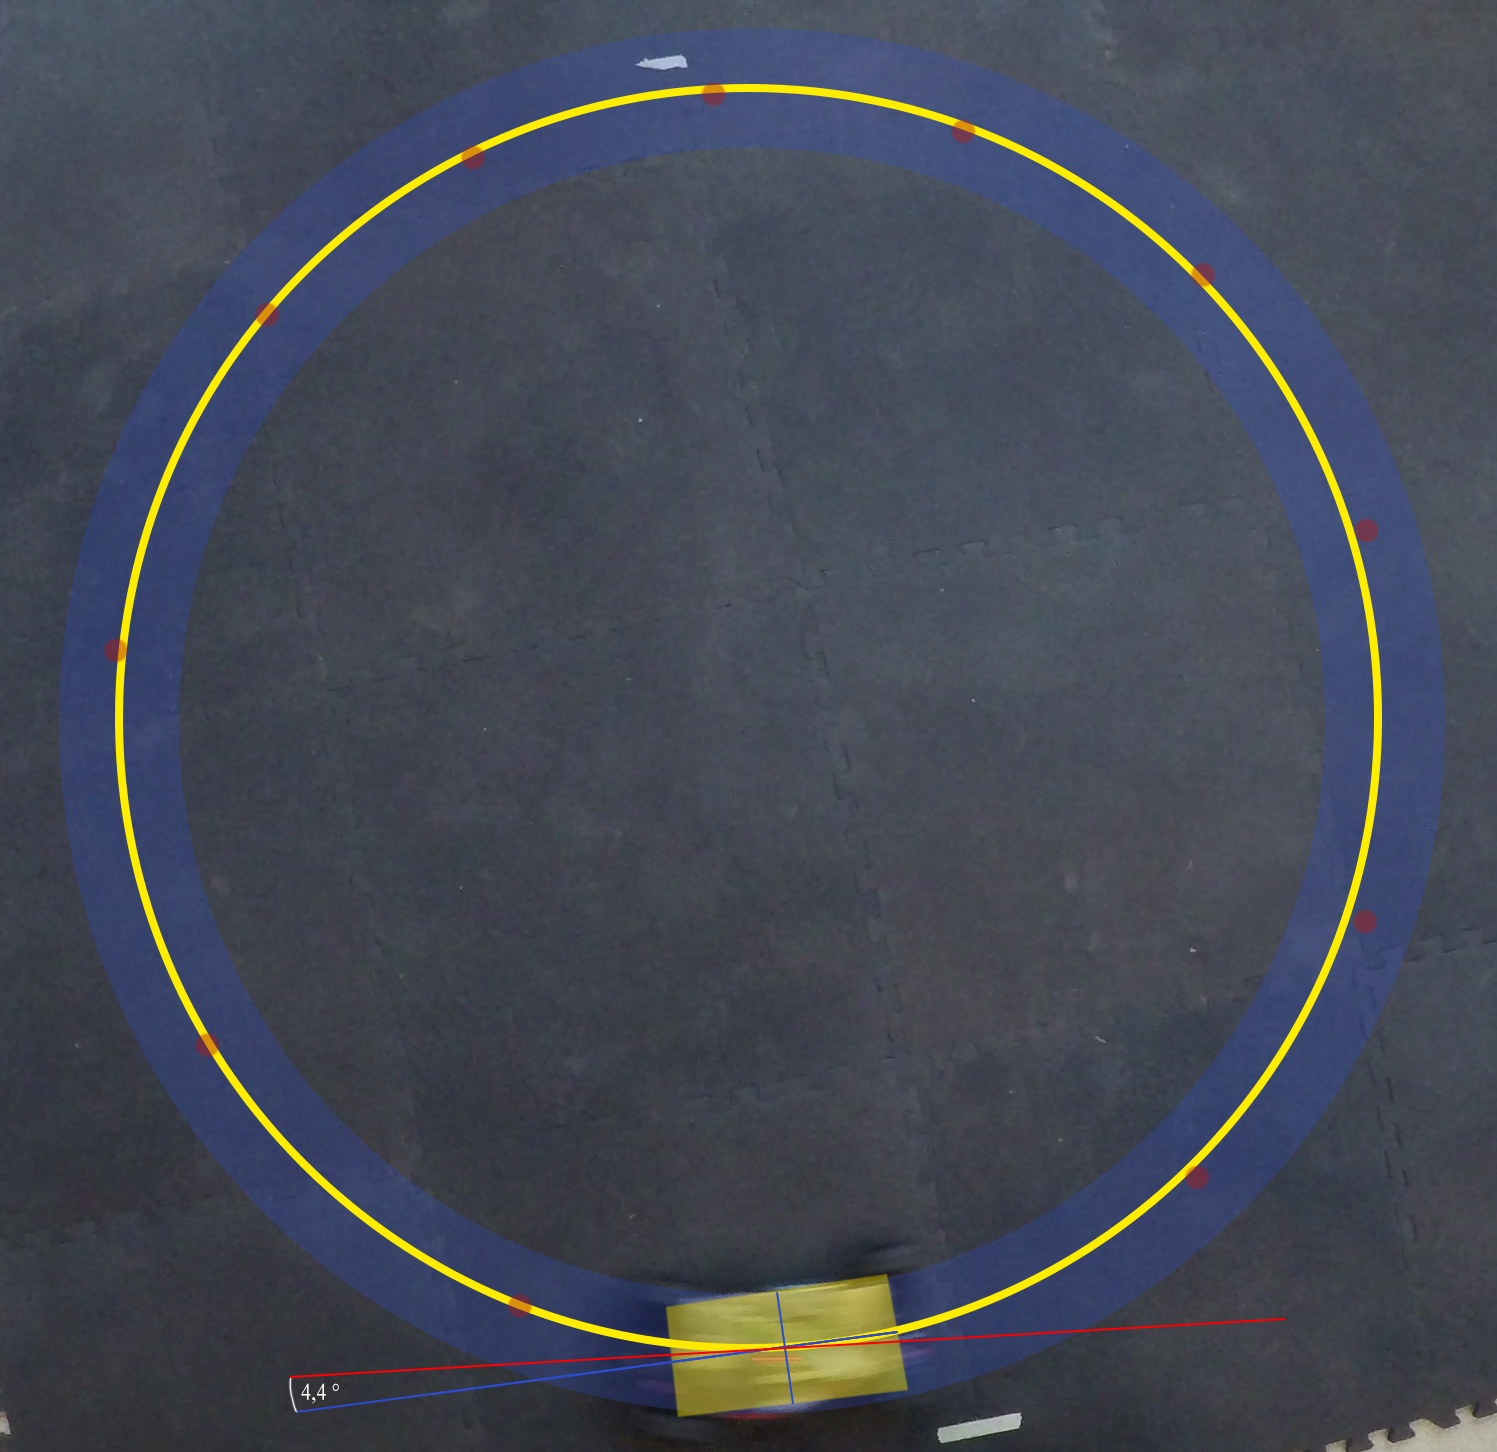
\includegraphics[scale=0.07]{Figures/Schwimmwinkel.png}
	\caption{Kreisfahrtwinkelanalyse}
	\label{fig:Kreis}
\end{subfigure}
\end{figure}
\end{center}\vspace{-0.7cm}
Somit sind Seitenkraftbeiwerte mit $28<k_{SH}<75$ und $15<k_{SV}<25$ denkbar. Da $k_{SH}l_H-k_{SV}l_V$ in jedem Fall positiv ist, spricht dies auch für ein Untersteuern des Fahrzeuges.
%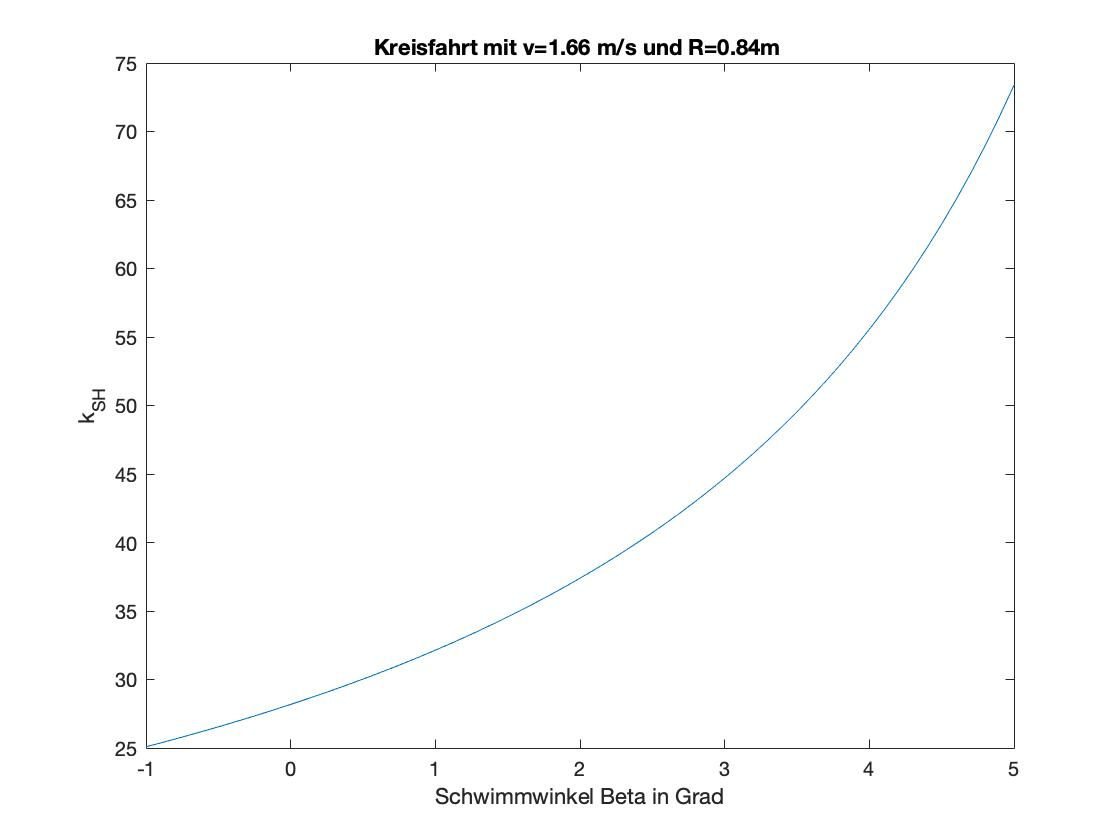
\includegraphics[scale=0.3]{ksh(beta).jpg}\\
%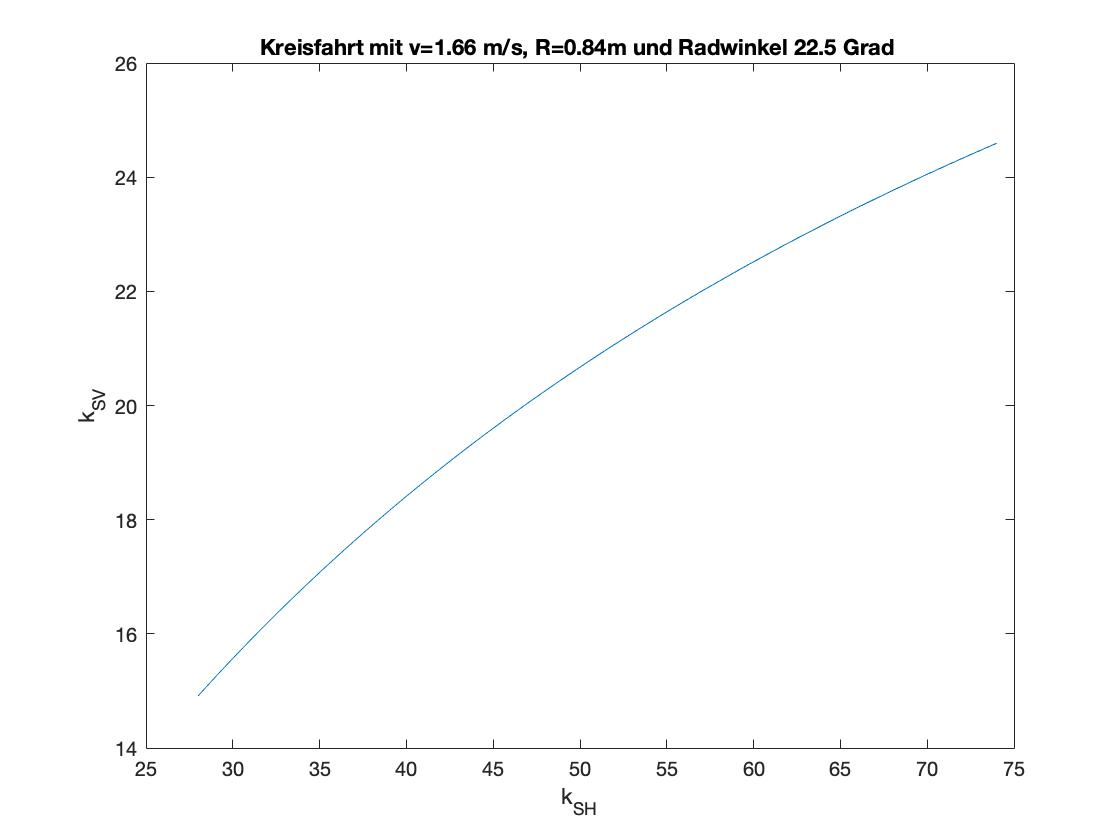
\includegraphics[scale=0.3]{ksv(ksv).jpg}
\end{document}
